\begin{enumerate}
\item Nineteen immigrants to the U.S. were asked how many years, to the nearest year, they have lived in the U.S.  The data are as follows: 
\begin{align*}
&2,\ 5,\ 7,\ 2,\ 2,\ 10,\ 20,\ 15,\ 0,\\ 
7,\ &0,\ 20,\ 5,\ 12,\ 15,\ 12,\ 4,\ 5,\ 10
\end{align*} 
Draw a dot plot to summarize this data.

\begin{center}
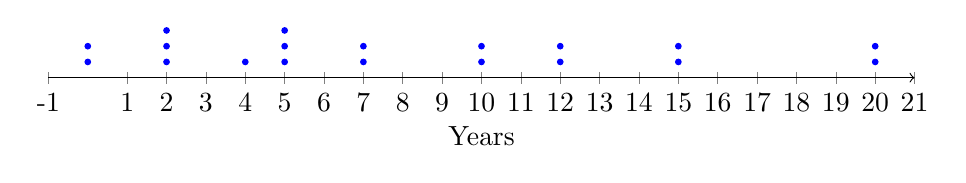
\begin{tikzpicture}
\begin{axis}[
    xmin=-1, xmax=21,
    ymin=0, ymax=5,
    axis lines=center,
    axis on top=false,
    domain=0:1,
    x=0.5cm,
    y=0.2cm,
    xtick={-1,0,...,21},
    xticklabels={-1,0,...,21},
    axis y line=none,
    ytick={},
    yticklabels={},
    axis lines=middle,
    axis line style={->},
    x label style={at={(axis description cs:0.5,-0.5)},anchor=north},
    y label style={at={(axis description cs:-0.1,.5)},rotate=90,anchor=south},
    xlabel={Years},
    ylabel={},
    grid=none
    ]
	\addplot [blue,only marks,mark size=1] table {
	0 1
	0 2
	2 1
	2 2
	2 3
	4 1
	5 1
	5 2
	5 3
	7 1
	7 2
	10 1
	10 2
	12 1
	12 2
	15 1
	15 2
	20 1
	20 2
	};
\end{axis}
\end{tikzpicture}
\end{center}

\item A group of students earned the following final grades:
\begin{center}
B, C, A, B, B, D, C, C, C, F, A, C, B, B, B, C, B, D
\end{center}
Draw a dot plot to summarize this data.

\begin{center}
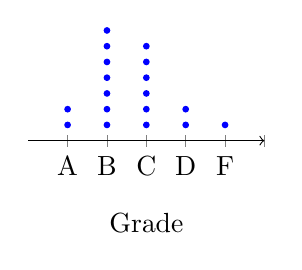
\begin{tikzpicture}
\begin{axis}[
    xmin=0, xmax=6,
    ymin=0, ymax=8,
    axis lines=center,
    axis on top=false,
    domain=0:1,
    x=0.5cm,
    y=0.2cm,
    xtick={0,1,...,6},
    xticklabels={N, A, B, C, D, F},
    axis y line=none,
    ytick={},
    yticklabels={},
    axis lines=middle,
    axis line style={->},
    x label style={at={(axis description cs:0.5,-0.5)},anchor=north},
    y label style={at={(axis description cs:-0.1,.5)},rotate=90,anchor=south},
    xlabel={Grade},
    ylabel={},
    grid=none
    ]
	\addplot [blue,only marks,mark size=1] table {
	1 1
	1 2	
	2 1
	2 2
	2 3
	2 4
	2 5
	2 6
	2 7
	3 1
	3 2
	3 3
	3 4
	3 5
	3 6
	4 1
	4 2
	5 1
	};
\end{axis}
\end{tikzpicture}
\end{center}

\item A store tracked how many iPads were sold each day for fifty days, and their data is below.
\begin{center}
\begin{tabular}{c c c c c c c c c c}
4 & 2 & 3 & 2 & 5 & 5 & 1 & 3 & 3 & 2\\
3 & 2 & 2 & 3 & 2 & 2 & 2 & 3 & 0 & 1\\
3 & 1 & 1 & 5 & 4 & 1 & 2 & 4 & 3 & 5\\
2 & 0 & 0 & 3 & 2 & 3 & 3 & 3 & 2 & 2\\
0 & 4 & 2 & 4 & 3 & 1 & 1 & 4 & 0 & 1
\end{tabular}
\end{center}
Construct a frequency table (including a relative frequency column) to describe this data.

\begin{center}
\begin{tabular}{c c c}
\textbf{iPads Sold} & \textbf{Frequency} & \textbf{Relative Frequency}\\
\hline
& & \\
0 & 5 & 0.10\\
1 & 8 & 0.16\\
2 & 14 & 0.28\\
3 & 13 & 0.26\\
4 & 6 & 0.12\\
5 & 4 & 0.08
\end{tabular}
\end{center}
\vfill
\pagebreak

\item Twenty students were asked how many hours they worked per day.  Their responses are as follows:
\begin{center}
\begin{tabular}{c c c c}
5 & 6 & 3 & 3\\
2 & 4 & 7 & 5\\
2 & 3 & 5 & 6\\
5 & 4 & 4 & 3\\
5 & 2 & 5 & 3
\end{tabular}
\end{center}
Construct a frequency table (including a relative frequency column) to describe this data.

\begin{center}
\begin{tabular}{c c c}
\textbf{Hours} & \textbf{Frequency} & \textbf{Relative Frequency}\\
\hline
& & \\
2 & 3 & 0.15\\
3 & 5 & 0.25\\
4 & 3 & 0.15\\
5 & 6 & 0.30\\
6 & 2 & 0.10\\
7 & 1 & 0.05
\end{tabular}
\end{center}

\item Fifty part-time students were asked how many courses they were taking this semester. The (incomplete) results are shown below. Fill in the blank cells to complete the table.
\begin{center}
\begin{tabular}{c c c }
\textbf{Number of Courses} & \textbf{Frequency} & \textbf{Relative Frequency}\\
\hline
& & \\
1 & 30 & 0.6\\
2 & 15 & {\LARGE\color{red}\bfseries 0.3}\\
3 & {\LARGE\color{red}\bfseries 5} & {\LARGE\color{red}\bfseries 0.1}
\end{tabular}
\end{center}

\item A group of 20 students were polled and asked what year they belonged to, whether they were freshmen (FR), sophomores (SO), juniors (JR), or seniors (SR).  The results are written below.\begin{center}
\begin{tabular}{c c c c}
FR & JR & SO & JR\\
SR & FR & SO & SO\\
SO & SR & SO & SR\\
SR & FR & SR & SO\\
SR & SO & JR & JR
\end{tabular}
\end{center}
Construct a frequency table (including a relative frequency column) to describe this data.

\begin{center}
\begin{tabular}{c c c}
\textbf{Year} & \textbf{Frequency} & \textbf{Relative Frequency}\\
\hline
& & \\
FR & 3 & 0.15\\
SO & 7 & 0.35\\
JR & 4 & 0.20\\
SR & 6 & 0.30
\end{tabular}
\end{center}

\item A group of 20 registered voters were polled and asked what party they belonged to, whether they were Republicans (R), Democrats (D), Green Party members (G), or independent (I).  The results are written below.\begin{center}
\begin{tabular}{c c c c}
R & R & D & D\\
G & D & R & D\\
I & R & R & D\\
I & D & R & I\\
R & D & R & D
\end{tabular}
\end{center}
Construct a frequency table (including a relative frequency column) to describe this data.

\begin{center}
\begin{tabular}{c c c}
\textbf{Party} & \textbf{Frequency} & \textbf{Relative Frequency}\\
\hline
& & \\
R & 8 & 0.40\\
D & 8 & 0.40\\
G & 1 & 0.05\\
I & 3 & 0.15
\end{tabular}
\end{center}

\item The following is the average daily temperature for Frederick, Maryland for the month of June: \begin{align*}74, 60, 58, 58, 64, 67, 64, 74, 72, 70,\\ 78, 80, 80, 79, 80, 80, 70, 83, 76, 78,\\ 81, 78, 81, 70, 70, 71, 66, 66, 68, 74.\end{align*}
\begin{enumerate}[(a)]
\item Construct a grouped frequency and relative frequency distribution using a class width of 5, starting at 55.

\begin{center}
\begin{tabular}{c c c}
\textbf{Temperature} & \textbf{Frequency} & \textbf{Relative Frequency}\\
\hline
& & \\
55--59 & 2 & 0.07\\
60--64 & 3 & 0.10\\
65--69 & 4 & 0.13\\
70--74 & 9 & 0.30\\
75--79 & 5 & 0.17\\
80--84 & 7 & 0.23
\end{tabular}
\end{center}

\item Construct a histogram from the frequency distribution. 

\begin{center}
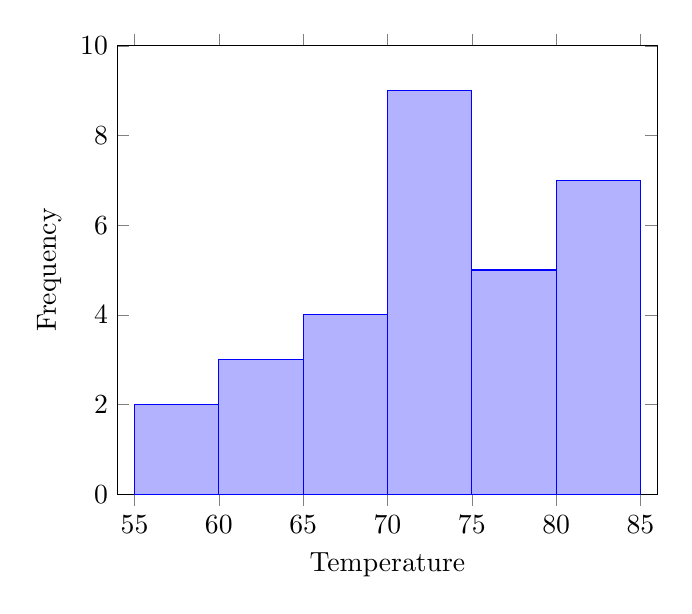
\begin{tikzpicture}
\begin{axis}[
	x tick label style={
		/pgf/number format/1000 sep=},
	ylabel={Frequency},
	xlabel={Temperature},
	legend style={at={(0.5,-0.1)},
	anchor=north,legend columns=-1},
	ybar,
	bar width=15pt,
	ymin=0,
	ymax=10,
	xmin=54,
	xmax=86,
	xtick=data,
	yticklabel style={
        /pgf/number format/fixed,
        /pgf/number format/precision=0
	},
	xticklabel style={
        /pgf/number format/fixed,
        /pgf/number format/precision=0
	},
]
\addplot+[ybar interval] plot 
	coordinates {(55,2) (60,3) (65,4)
		 (70,9) (75,5) (80,7) (85,0) };
\end{axis}
\end{tikzpicture}
\end{center}

\end{enumerate}

\item A researcher gathered data on hours of video games played by school-aged children and young adults. She collected the following data: \begin{align*}0, 0, 1, 1, 1, 2, 2, 3, 3, 3,\\ 4, 4, 4, 4, 5, 5, 5, 6, 6, 7,\\ 7, 7, 8, 8, 8, 8, 8, 9, 9, 9,\\ 10, 10, 11, 12, 12, 12, 12, 13. \end{align*}
\begin{enumerate}[(a)]
\item Construct a grouped frequency and relative frequency distribution using a class width of 2, starting at 0.

\begin{center}
\begin{tabular}{c c c}
\textbf{Temperature} & \textbf{Frequency} & \textbf{Relative Frequency}\\
\hline
& & \\
0--1 & 5 & 0.13\\
2--3 & 5 & 0.13\\
4--5 & 7 & 0.18\\
6--7 & 5 & 0.13\\
8--9 & 8 & 0.21\\
10-11 & 3 & 0.08\\
12-13 & 5 & 0.13
\end{tabular}
\end{center}
\pagebreak

\item Construct a histogram from the frequency distribution. 

\begin{center}
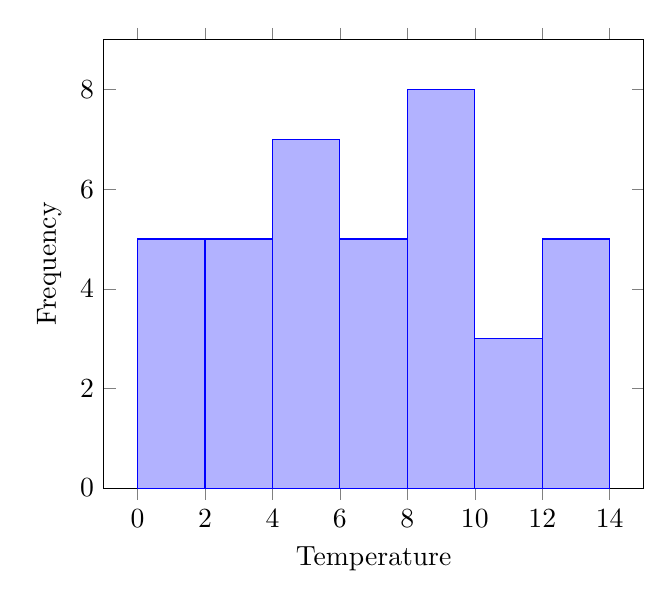
\begin{tikzpicture}
\begin{axis}[
	x tick label style={
		/pgf/number format/1000 sep=},
	ylabel={Frequency},
	xlabel={Temperature},
	legend style={at={(0.5,-0.1)},
	anchor=north,legend columns=-1},
	ybar,
	bar width=15pt,
	ymin=0,
	ymax=9,
	xmin=-1,
	xmax=15,
	xtick=data,
	yticklabel style={
        /pgf/number format/fixed,
        /pgf/number format/precision=0
	},
	xticklabel style={
        /pgf/number format/fixed,
        /pgf/number format/precision=0
	},
]
\addplot+[ybar interval] plot 
	coordinates {(0,5) (2,5) (4,7)
		 (6,5) (8,8) (10,3) (12,5) (14,0) };
\end{axis}
\end{tikzpicture}
\end{center}

\end{enumerate}
\end{enumerate}

\emph{For exercises 10--13, use the frequency table below, which contains the total number of deaths worldwide as a result of earthquakes for the period from 2000 to 2012.}
\begin{center}
\begin{tabular}{c c}
\textbf{Year} & \textbf{Total Number of Deaths}\\
\hline
& \\
2000 & 231\\
2001 & 21,357\\
2002 & 11,685\\
2003 & 33,819\\
2004 & 228,802\\
2005 & 88,003\\
2006 & 6,605\\
2007 & 712\\
2008 & 88,011\\
2009 & 1,790\\
2010 & 320,120\\
2011 & 21,953\\
2012 & 768\\
\textbf{Total} & \textbf{823,356}
\end{tabular}
\end{center}

\begin{enumerate}
\setcounter{enumi}{9}
\item What is the frequency of deaths measured from 2006 through 2009? \answer{97,118}
\[6,605 + 712 + 88,011 + 1,790 = 97,118\]

\item What percentage of deaths occurred after 2009 (from 2010 onwards)? \answer{41.6\%}
\[320,120 + 21,953 + 768 = 342,841 \longrightarrow \dfrac{342,841}{823,356} = 0.416\]

\item What is the relative frequency of deaths that occurred in 2003 or earlier? \answer{0.081 or 8.1\%}
\[231 + 21,357 + 11,685 + 33,819 = 67,092 \longrightarrow \dfrac{67,092}{823,356} = 0.081\]

\item What is the percentage of deaths that occurred in 2004? \answer{27.8\%}
\[\dfrac{228,802}{823,356} = 0.278\]

\item What is wrong with the following grouped frequency distribution?
\begin{center}
\begin{tabular}{c | c}
\textbf{Grades} & \textbf{Frequency}\\
\hline
50--55 & 2\\
55--60 & 4\\
60--70 & 9\\
70--80 & 15\\
80--90 & 7\\
90 and above & 4
\end{tabular}
\end{center}
\begin{enumerate}[(a)]
\item The classes do not all have the same width.
\item The classes overlap.
\item There are open-ended classes.
\item All of the above.
\end{enumerate} \text{} \answer{(d) All of the above}

\item Draw a bar chart for the dataset in problem 6.

\begin{center}
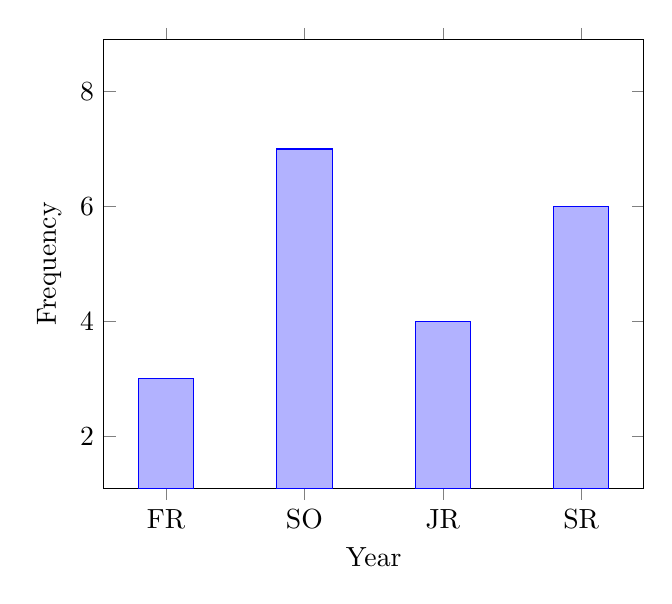
\begin{tikzpicture}
\begin{axis}[
	x tick label style={
		/pgf/number format/1000 sep=},
	ylabel={Frequency},
	xlabel={Year},
	xticklabels={,,FR,SO,JR,SR},
	yticklabels={,0,2,4,6,8},
	enlargelimits=0.15,
	legend style={at={(0.5,-0.1)},
	anchor=north,legend columns=-1},
	ybar,
	bar width=20pt,
	ymin=2,
	ymax=8,
	%nodes near coords,
	%nodes near coords style={
	%	/pgf/number format/.cd,fixed zerofill,precision=1},
	%nodes near coords align={vertical},
]
\addplot 
	coordinates {(1,3) (2,7)
		 (3,4) (4,6)};
\end{axis}
\end{tikzpicture}
\end{center}

\item Draw a bar chart for the dataset in problem 7.

\begin{center}
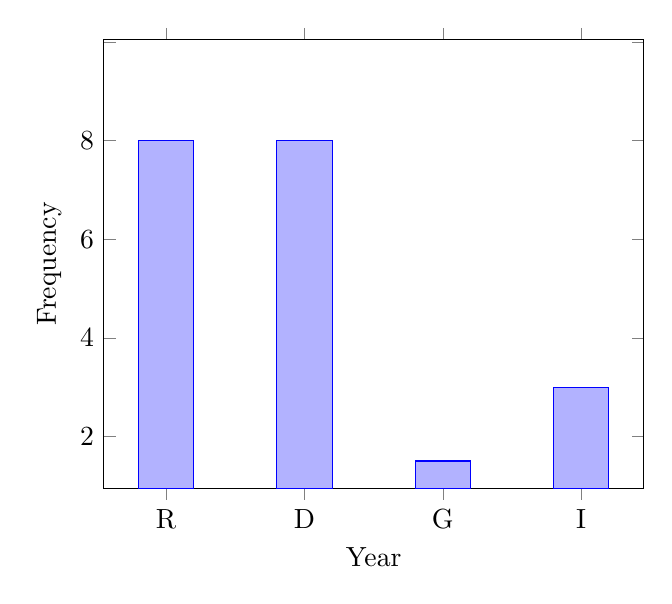
\begin{tikzpicture}
\begin{axis}[
	x tick label style={
		/pgf/number format/1000 sep=},
	ylabel={Frequency},
	xlabel={Year},
	xticklabels={,,R,D,G,I},
	yticklabels={,0,2,4,6,8},
	enlargelimits=0.15,
	legend style={at={(0.5,-0.1)},
	anchor=north,legend columns=-1},
	ybar,
	bar width=20pt,
	ymin=2,
	ymax=9,
	%nodes near coords,
	%nodes near coords style={
	%	/pgf/number format/.cd,fixed zerofill,precision=1},
	%nodes near coords align={vertical},
]
\addplot 
	coordinates {(1,8) (2,8)
		 (3,1.5) (4,3)};
\end{axis}
\end{tikzpicture}
\end{center}
\pagebreak

\item The scores for a math test are shown below, ordered from smallest to largest.
\begin{center}
\begin{tabular}{c c c c c c}
42 & 49 & 49 & 53 & 55 & 55\\
61 & 63 & 67 & 68 & 68 & 69\\
69 & 72 & 73 & 74 & 78 & 80\\
83 & 88 & 88 & 88 & 90 & 92\\
94 & 94 & 94 & 95 & 96 & 100
\end{tabular}
\end{center}
Build a stem-and-leaf plot for this data.

\begin{center}
\begin{tabular}{r | l}
Stems & Leaves\\
\hline
4 & 2 9 9\\
5 & 3 5 5\\
6 & 1 3 7 8 8 9 9\\
7 & 2 3 4 8\\
8 & 0 3 8 8 8\\
9 & 0 2 4 4 4 5 6\\
10 & 0
\end{tabular}
\end{center}

\item A basketball team's scores for the last 30 games are shown below, ordered from smallest to largest.
\begin{center}
\begin{tabular}{c c c c c c}
32 & 32 & 33 & 34 & 38 & 40\\
42 & 42 & 43 & 44 & 46 & 47\\
47 & 48 & 48 & 48 & 49 & 50\\
50 & 51 & 52 & 52 & 52 & 53\\
54 & 56 & 57 & 57 & 60 & 61
\end{tabular}
\end{center}
Build a stem-and-leaf plot for this data.

\begin{center}
\begin{tabular}{r | l}
Stems & Leaves\\
\hline
3 & 2 2 3 4 8\\
4 & 0 2 2 3 4 6 7 7 8 8 8 9\\
5 & 0 0 1 2 2 2 3 4 6 7 7\\
6 & 0 1
\end{tabular}
\end{center}

\item The following stem-and-leaf plots compare the ages of 30 actors and 30 actresses at the time they won the Oscar award for Best Actor or Actress.
\begin{center}
\begin{tabular}{|r | c | l|}
\hline
Actors & Stems & Actresses\\
\hline
& 2 & 146667\\
\hline
98753221 & 3 & 00113344455778\\
\hline
88776543322100 & 4 & 11129\\
\hline
6651 & 5 & \\
\hline
210 & 6 & 011\\
\hline
6 & 7 & 4\\
\hline
& 8 & 0\\
\hline
\end{tabular}
\end{center}
\begin{enumerate}[(a)]
\item What is the age of the youngest actor to win an Oscar? \answersub{31 years}

\item What is the age difference between the oldest and the youngest actress to win an Oscar? \answersub{59 years}
\[80 - 21 = 59\]

\item What is the oldest age shared by two actors to win an Oscar? \answersub{56 years}
\end{enumerate}
\pagebreak

\item The table below shows the yearly tuition of 8 universities, as well as the average mid-career salaries for graduates of each university.
\begin{center}
\begin{tabular}{l c c}
\textbf{University} & \textbf{Tuition (\$)} & \textbf{Salary (\$)}\\
\hline
& & \\
Princeton & 28,540 & 137,000\\
Harvey Mudd & 40,133 & 135,000\\
CalTech & 39,900 & 127,000\\
MIT & 42,050 & 118,000\\
Lehigh University & 43,220 & 118,000\\
NYU-Poly & 39,565 & 117,000\\
Babson College & 40,400 & 117,000\\
Stanford & 54,506 & 114,000
\end{tabular}
\end{center}
Draw a scatterplot for this data, using $x$ to represent tuition and $y$ to represent salary.

\begin{center}
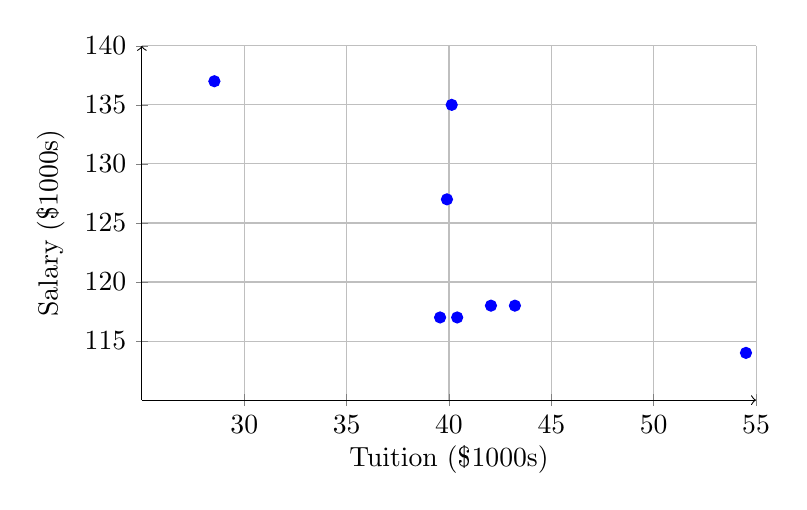
\begin{tikzpicture}
\begin{axis}[
    xmin=25, xmax=55,
    ymin=110, ymax=140,
    axis lines=center,
    axis on top=false,
    domain=0:1,
    x=0.26cm,
    y=0.15cm,
    xtick={25,30,...,55},
    xticklabels={25,30,...,55},
    ytick={110,115,...,140},
    yticklabels={110,115,...,140},
    axis lines=middle,
    axis line style={->},
    x label style={at={(axis description cs:0.5,-0.1)},anchor=north},
    y label style={at={(axis description cs:-0.11,.5)},rotate=90,anchor=south},
    xlabel={Tuition (\$1000s)},
    ylabel={Salary (\$1000s)},
    grid=major
    ]
	\addplot [blue,only marks,mark size=2] table {
	28.54 137
	40.133 135
	39.9 127
	42.05 118
	43.22 118
	39.565 117
	40.4 117
	54.506 114
	};
\end{axis}
\end{tikzpicture}
\end{center}

\item The table below shows the frequency of chirps for the striped ground cricket compared to the ambient temperature.
\begin{center}
\begin{tabular}{c c}
\textbf{Chirps per Second} & \textbf{Temperature ($^\circ$F)}\\
\hline
& \\
20.0 & 88.6\\
16.0 & 71.6\\
19.8 & 93.3\\
18.4 & 84.3\\
17.1 & 80.6\\
15.5 & 75.2\\
14.7 & 69.7\\
17.1 & 82.0\\
15.4 & 69.4
\end{tabular}
\end{center}
Draw a scatterplot for this data, using $x$ to represent the chirping frequency and $y$ to represent temperature.

\begin{center}
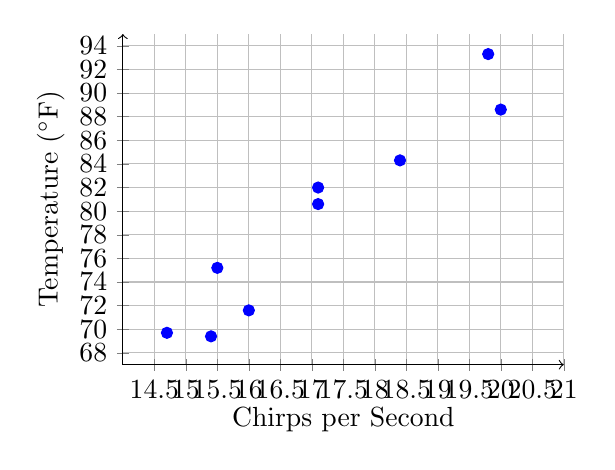
\begin{tikzpicture}
\begin{axis}[
    xmin=14, xmax=21,
    ymin=67, ymax=95,
    axis lines=center,
    axis on top=false,
    domain=0:1,
    x=0.8cm,
    y=0.15cm,
    xtick={14,14.5,...,21},
    xticklabels={14,14.5,...,21},
    ytick={68,70,...,94},
    yticklabels={68,70,...,94},
    axis lines=middle,
    axis line style={->},
    x label style={at={(axis description cs:0.5,-0.1)},anchor=north},
    y label style={at={(axis description cs:-0.11,.5)},rotate=90,anchor=south},
    xlabel={Chirps per Second},
    ylabel={Temperature ($^\circ$F)},
    grid=major
    ]
	\addplot [blue,only marks,mark size=2] table {
	20.0 88.6
	16.0 71.6
	19.8 93.3
	18.4 84.3
	17.1 80.6
	15.5 75.2
	14.7 69.7
	17.1 82.0
	15.4 69.4
	};
\end{axis}
\end{tikzpicture}
\end{center}

\end{enumerate}